\chapter{State of the Art}
\label{chap:enabling_technologies}
This chapter will serve as a compilation of past work in automatic sarcasm detection.
Firstly, a brief introduction to the main learning technologies used for text-based learning will be given. Moreover, an analysis of automatic sarcasm detection will be briefed. Finally, the main issues found in automatic sarcasm detection shall be overviewed.

\section{Introduction}
Sarcasm detection is an important component for~\ac{nlp} very relevant to natural language understanding, dialogue systems and text mining~\cite{khodak2017large}.\\ The perspective followed in this chapter is merely to give a glimpse to the reader of the state-of-the-art technologies used by other researchers in this field. \\
The chapter will begin by defining sarcasm and its context. 
\section{Sarcasm} 
\subsection{Sarcasm Definition~\cite{joshi2017automatic}}
The Free Dictionary\footnote{www.thefreedictionary.com} defines sarcasm as a form of verbal irony that is intended to express contempt or ridicule. The subjective characteristic of sarcasm makes sarcasm very difficult to detect since a word may have a literal meaning and a sarcastic meaning. As a result, sarcasm automatic detection presents a big challenge. \\
Typically, sarcasm detection has been formulated as a classification problem. In that sense, given text, the goal is to predict whether or not the text is sarcastic. However, the big challenge is to label the text, since the classifier is supposed to distinguish between irony,  humour and other sentimental meanings.\\
In linguistics, sarcasm is a form of figurative language where the literal meaning of words does not hold, and instead, the opposite interpretation is intended. Sarcasm is a type of irony. 

\section{Dataset~\cite{joshi2017automatic}}

As a matter of a fact, the studies already done in automatic sarcasm detection depend entirely on the dataset. That is why it is convenient to divide them into three kinds:
\begin{itemize}
	\item \textit{Short texts}: The social network Twitter is extremely popular due to its popularity among users. It can serve as an example of short text since every tweet is restricted to not exceed a certain number of words. One approach to obtaining labels for the tweets is to manually mark them as sarcastic or non-sarcastic. Another approach is hashtag-based supervision. Hashtags can reveal when a tweet is labelled as sarcastic. By introducing the \textit{sarcasm} label, the author makes clear his intention to use sarcasm.  This allows the dataset to be bigger. Many works using this variation have been reported since its popularity has constantly grown. One of the problems with Twitter is the text length restriction. If the tweet length exceeds the tweet restriction limit, the author is going to be forced to introduce abbreviations to the words used. As a consequence, sarcasm detection is going to be harder since the words are not going to be correctly spelt.
	\item \textit{Long texts}: The information usually comes from reviews, posts, news, articles. Some of the popular platforms for sentiment analysis in long texts are imdb (for film critiques) and reddit. 
	\item \textit{Other data-sets}
\end{itemize}

It is noteworthy to mention the emphasis made on the Twitter social network since this project will be focusing on a Spanish set of tweets to detect sarcasm. Please note that this project will be developed for short texts. Hence, all the conclusions made are only valid for short texts.

\section{Approaches used for Sarcasm Detection}
\label{sec:sarcasmapproach}
In this section, several approaches used for detecting sarcasm will be discussed. In general, approaches for sarcasm detection can be classified into rule-based, statistical and deep learning-based approaches~\cite{joshi2017automatic}.
\subsection{Rule-based Approaches~\cite{joshi2017automatic}}
Rule-based approaches work by identifying sarcasm through a set of rules based upon evidence. The evidence is captured by using rules relying upon sarcasm. For instance, one rule can rely on Google to determine how likely that smile (emoticon) is while another rule can come from hashtag analysis. By identifying the hashtags present in a tweet, a sarcasm pattern could be found. If the sentiment detected in the tweet does not match with the hashtag, then that tweet is labelled as sarcastic.\\ Furthermore, one could find sarcasm if a positive verb happens in a negative situation phrase in a sentence. The problem here is extracting the set of negative situation phrases. This is also known as a rule-based approach.
\subsection{Feature sets \cite{joshi2017automatic}}
This kind of approach used some of the technologies described below. In this project, there was a combination of features and learning algorithms but, in contrast, no deep learning technologies were implemented.
\begin{itemize}
	\item \textit{Features Used:} Most of these approaches use bag-of-words as features that have been found by statistical sarcasm detection. Apart from finding the features, some other works focus on designing pattern-based features, that are able to indicate sarcastic patterns on the corpus. The majority of the features used can be found in~\cref{fig:featused}. To allow the classifier to spot sarcastic patterns, these pattern-based features take three real values: exact match, partial match and no match. Furthermore, pragmatic features, like emoticons, can also be considered. For the sake of simplicity, the contextual sarcastic features (i.e. features that depend on previous messages) are not considered in this project.
	\item \textit{Learning Algorithms:} A variety of classifiers have already experimented for sarcasm detection.~\acf{svm} is quite often present in sarcasm detection classification techniques. Moreover, many other works have used~\acf{lr},~\acf{nb} and Random Forests.
	\item \textit{Deep Learning-based Approaches:} Although nowadays deep learning has raised a lot of awareness, there are still few approaches reported for automated sarcasm detection. A similarity between word embeddings as features for sarcasm detection has been reported. This augments features based on similarity of word embeddings related to other word pairs and report an improvement on performance. Convolutional neural networks have also been implemented, reporting an improvement of $2\%$ in performance.
\end{itemize}
\begin{figure}
	\centering
	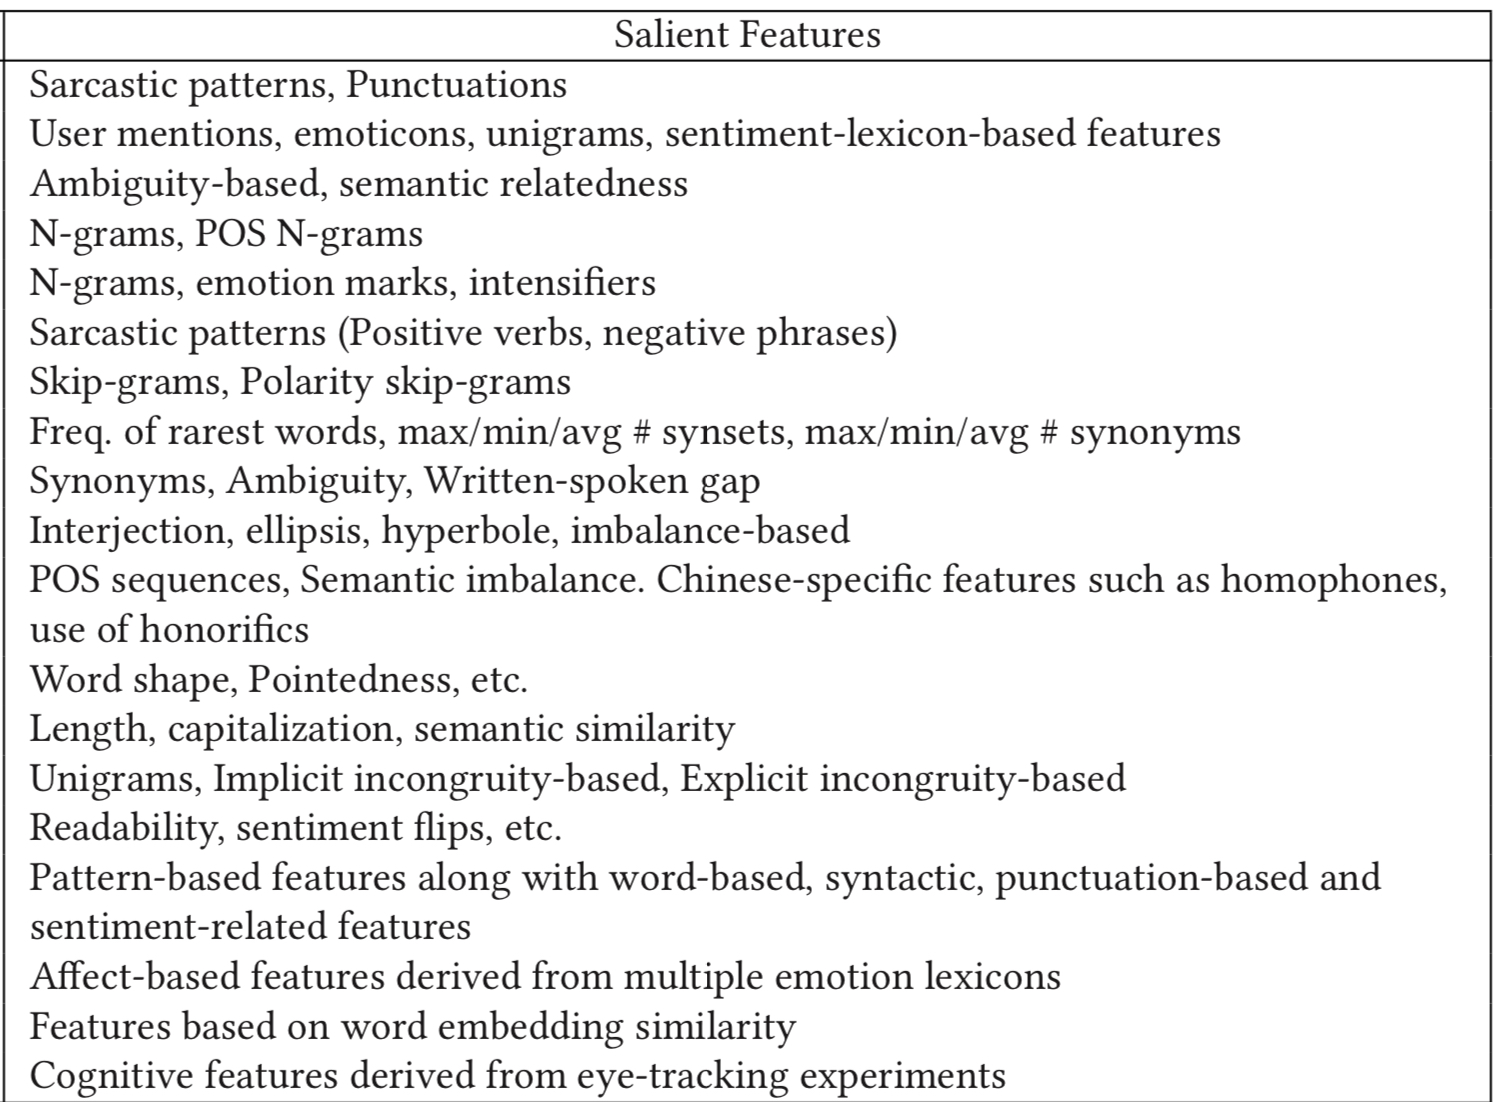
\includegraphics[scale=0.25]{img/features.jpeg}
	\caption{Features used for Statistical Classifiers~\cite{joshi2017automatic}}
	\label{fig:featused}
\end{figure}
To put it in a nutshell, different techniques for automatic sarcasm detection can be performed. Despite these numerous techniques, sarcasm automatic detection is difficult to detect since a word can have a literal meaning but also a sarcastic meaning that is not so easily labelled.

\section{Main Issues in Sarcasm Detection}
There are three main issues present in sarcasm automatic detection techniques~\cite{joshi2017automatic}:
\begin{itemize}
	\item \textit{Data:} Even though hashtag-based labelling can provide large-scale supervision, the quality of the dataset can be doubtful. For example, let us take the hashtag \textit{\#not} very often present in tweets. Is this supposed to express sarcasm in the sentence or is it simply used to express a negation? In most of the works, this problem is tackled by removing the \textit{\#not} in the pre-processing step and analyzing the sentence. However, this may as well not be the optimum solution. Another solution is to use as test set some manually labelled tweets and as train set a hashtag labelled set. 
	\item \textit{Features as Sentiment:} The question is how can sentiment be detected in a sentence? In the case of sarcasm, some answers have already been given. If a negative phrase occurs in a positive sentence then that sentence has most likely sarcasm. In a statistical classifier, surface polarity can be used as a feature of the tweet. To capture surface polarity one has to analyze two emotions: activation and pleasantness. This can lead to a $4\%$ improvement in the accuracy~\cite{joshi2017automatic}.
	\item \textit{Skewed Data-sets: }
	Sarcasm is hard to find in an expression. For that reason, skew is reflected in data-sets.
\end{itemize}

\section{Figures of Merit}
This section is committed to showing other past works in Sarcasm Detection for tweets. The decisive parameters shown in this section will be the F-measure.

\begin{itemize}
	\item Sarcasm Detection on Czech and English Twitter~\cite{ptavcek2014sarcasm}:
	\begin{itemize}
		\item \textit{Description}: This paper presents a \ac{ml} approach to sarcasm detection on Twitter in two languages - English and Czech. The classification was carried out by using~\ac{svm} classifiers and Maximum Entropy. Since only \ac{svm} has been implemented in this project, the latter will be discarded.
		\item \textit{Results:} F-measure (balanced dataset):~\textbf{0.947}. F-measure (unbalanced dataset):~\textbf{0.924}. Algorithm:~\textbf{\ac{svm}}
	\end{itemize}
	\item Irony detection in short texts~\cite{mexic}:
	\begin{itemize}
		\item \textit{Description}: This docuemnt summarizes the result of analyzing ironic tweets. The language is spanish.
		\item \textit{Results:} F-measure (balanced dataset):~\textbf{0.86}. F-measure (unbalanced dataset):~\textbf{0.82}. Algorithm:~\textbf{\ac{svm}}
	\end{itemize}
	
\end{itemize}
Moreover, in~\cite{joshi2017automatic} a table can be found with a collection of many other past works in sarcasm detection. However, the values on the table are not directly comparable, because different datasets and techniques have been used by the authors.\\
\begin{table}
	\centering
	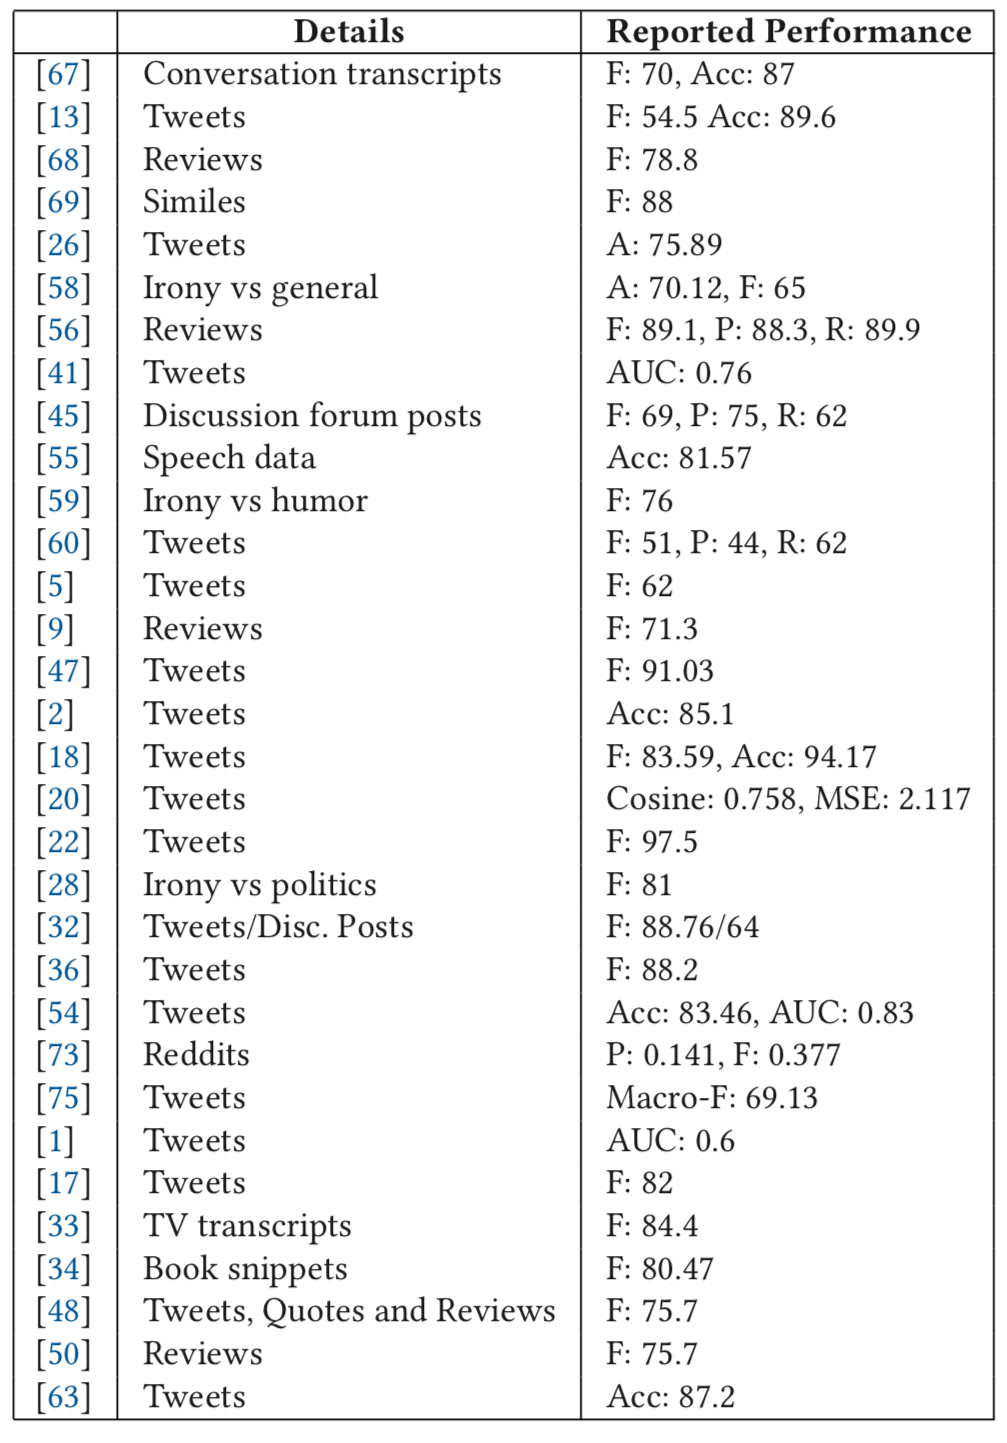
\includegraphics[scale=0.35]{img/performanceValues.jpeg}
	\caption{Performance Values of Sarcasm Detection; Precision/Recall/F-measures and Accuracy Values indicated in Percentages~\cite{joshi2017automatic}}
	\label{tab:performanceBench}
\end{table}
In the~\cref{tab:performanceBench} a compilation of performance values of sarcasm detection is shown.\\ 
The left column represents the citations used in the article~\cite{joshi2017automatic}. Therefore, they do not correspond to this projects' citations.\\
The middle column is expressing whether the dataset was composed of short texts, such as tweets, or other long texts, like reddits.\\
Finally, the third column shows the score achieved. To simplify, the F1 Score (in the table is represented as \textit{F}) will be considered the most relevant score. The average F1 Score is $76,771\%$. To compute the average, only tweets displaying a F1 Score in the table have been considered.\\
For more information on F1 Score see~\cref{sec:score}.